opencode%=================== Modificado por Elliot.C12 ======================
%=================== Basado en UPIITA ===========================
%=================== Plantilla de informe EPN ===================

\documentclass[12pt,a4paper]{article}
\title{Plantilla para trabajos}
\usepackage{STY/INICIO}
\usepackage{STY/slashbox}
%=================== Añade Otro nivel de sección ===================
\usepackage{titlesec}
\setcounter{secnumdepth}{4}
\titleformat{\paragraph}
{\normalfont\normalsize\bfseries}{\theparagraph}{1em}{}
\titlespacing*{\paragraph}
{0pt}{3.25ex plus 1ex minus .2ex}{1.5ex plus .2ex}

\makeatletter
\renewcommand\paragraph{\@startsection{paragraph}{4}{\z@}%
            {-2.5ex\@plus -1ex \@minus -.25ex}%
            {1.25ex \@plus .25ex}%
            {\normalfont\normalsize\bfseries}}
\makeatother
\setcounter{secnumdepth}{4} % how many sectioning levels to assign numbers to
\setcounter{tocdepth}{4}    % how many sectioning levels to show in ToC
%=================== Paquetes para DF ===================
\usepackage{tikz}
\usetikzlibrary{shapes.geometric, arrows}

\tikzstyle{startstop} = [rectangle, rounded corners, 
minimum width=3cm, 
minimum height=1cm,
text centered, 
draw=black, 
fill=red!30]
\tikzstyle{io} = [trapezium, 
trapezium stretches=true, % A later addition
trapezium left angle=70, 
trapezium right angle=110, 
minimum width=3cm, 
minimum height=1cm, text centered, 
draw=black, fill=blue!30]
\tikzstyle{process} = [rectangle, 
minimum width=3cm, 
minimum height=1cm, 
text centered, 
text width=3cm, 
draw=black, 
fill=orange!30]
\tikzstyle{decision} = [diamond, 
minimum width=3cm, 
minimum height=1cm, 
text centered, 
draw=black, 
fill=green!30]
\tikzstyle{arrow} = [thick,->,>=stealth]
%======================================
\asignatura{Desarrollo de Videojuegos - 30817} %Texto en la parte derecha abajo
\carrera{}
\titulo{Bounty Run EC Documentación }
\grupo{4}
\alumno{Gabriel López, Marcelo Pareja, Bryan Quispe}
\profesor{Ing. Daniel Pinto}
\begin{document}
\maketitlepage % Portada
\newpage


%=============================================================
%=================== Inicio del Documeunto ===================
%=============================================================

%=================== Indices ===================
%\tableofcontents %Índice
%\newpage
%\listoffigures   %Índice de figuras
%\newpage        
%\listoftables   %Índice de tablas
%\newpage
%=================== Cuerpo del Documento ===================
\section{Introducción}
En el desarrollo de software, garantizar la calidad del producto final es un aspecto fundamental para satisfacer las necesidades de los usuarios y asegurar su correcto funcionamiento en diferentes entornos. Se han propuesto diversos modelos de evaluación, entre los cuales, el modelo de calidad de Boehm, organiza características del software en diferentes niveles o capas, permitiendo analizar tanto aspectos generales como detalles técnicos y específicos.\\ \\
Este trabajo presenta una descripción estructurada de dichas características, clasificándolas en niveles de alto nivel, intermedio y primitivo, con el objetivo de comprender cómo cada una contribuye a la calidad global del software. Además, se analiza la relación entre estas capas y su importancia en la evaluación del producto.


\section{Desarrollo}

\subsection{Definición}
El modelo jerárquico de calidad de software fue propuesto por Barry Boehm en 1978, durante una etapa conocida como la “crisis del software”. En la década de 1970, el uso de sistemas informáticos crecía rápidamente en empresas, gobiernos y organizaciones, pero muchos proyectos presentaban errores, retrasos y altos costos de desarrollo. Esto generó la necesidad de crear métodos que permitieran evaluar y mejorar la calidad del software de manera más organizada.\\ \\
La motivación principal de Boehm fue establecer un modelo que ayudará a medir la calidad no solo desde el funcionamiento técnico del sistema, sino también considerando aspectos como la confiabilidad, eficiencia, facilidad de uso y mantenimiento. Su propuesta buscaba garantizar que el software cumpliera las necesidades reales de los usuarios y pudiera mantenerse correctamente con el paso del tiempo.\\ \\
El entorno tecnológico de esa época era muy diferente al actual. Los sistemas se desarrollaban principalmente para computadoras centrales (mainframes), con recursos limitados de hardware y procesos de programación secuenciales. Además, las metodologías ágiles y las prácticas modernas como DevOps aún no existían, por lo que la calidad se evaluaba principalmente al final del desarrollo. En este contexto, el modelo de Boehm representó un avance importante al introducir una visión estructurada y jerárquica de la calidad del software.


\subsection{Características por capas del modelo}

\subsubsection{Características de Alto nivel}
Las características de alto nivel, se conocen también como \textit{“objetivos globales de calidad”}, ya que son los criterios que usan los usuarios finales para evaluar la calidad de un producto de software. Como indica Boehm, al momento de adquirir un producto de software, se suelen formular tres preguntas:
\begin{enumerate}
    \item ¿Qué tan útil es?
    \item ¿Qué tan fácil es de mantener?
    \item ¿Se puede usar en un entorno diferente?
\end{enumerate}
Cada una de estas preguntas está relacionada a una característica de alto nivel.
\begin{itemize}
    \item \textbf{Utilidad:} Hace referencia al grado en que el software responde y satisface las necesidades del usuario. En inglés, se usa el término de utilidad “as-is”, lo que indica que el software debe ser capaz de ser usado con facilidad y cumplir las funciones planificadas en su \textit{estado original}, sin necesidad de cambios o mejoras.
    \item \textbf{Mantenibilidad:} Representa el esfuerzo o dificultad necesaria para realizar cambios en el software tras su lanzamiento, sean actualizaciones, mejoras o correcciones. 
    \item \textbf{Portabilidad:} Es la capacidad del software para ser adaptado a diferentes entornos: sistemas operativos, dispositivos y tecnologías, sin perder su funcionalidad.
\end{itemize}
\subsubsection{Características de Nivel Intermedio}
El nivel intermedio conecta las características de alto nivel con las primitivas (más específicas y técnicas). Sus atributos principales son: 
\begin{itemize}
    \item \textbf{Portabilidad:} Capacidad del software para ser transferido y ejecutado en diferentes entornos o plataformas sin grandes modificaciones.
    \item \textbf{Fiabilidad:} Probabilidad de que el sistema funcione correctamente bajo condiciones específicas durante un tiempo determinado.
    \item \textbf{Eficiencia:} Uso óptimo de recursos como memoria, tiempo de ejecución y capacidad de procesamiento.
    \item \textbf{Usabilidad:} Facilidad con la que los usuarios pueden aprender, entender y operar el sistema.
    \item \textbf{Capacidad de prueba (testabilidad):} Facilidad para diseñar y ejecutar pruebas que validen el correcto funcionamiento del software.
    \item \textbf{Comprensión (understandability):} Qué tan fácil es para los desarrolladores entender el código y la estructura del sistema.
    \item \textbf{Flexibilidad:} Posibilidad de modificar el software para adaptarlo a nuevas necesidades o requisitos.
\end{itemize}

\subsubsection{Características de Nivel primitivo}
Son características que se asocian a una o dos métricas de calidad, y a partir de ellas se crean factores medibles con los que calificar al software. Entre estos están agrupados por las características de nivel intermedio:

\begin{itemize}
    \item \textbf{Portabilidad} \begin{itemize}
        \item \textit{Independencia de dispositivos:} Capacidad del software de funcionar en cualquier dispositivo
        \item \textit{Autocontención}
    \end{itemize}
    \item \textbf{Confiabilidad} \begin{itemize}
        \item \textit{Completitud} Todos los módulos de software están en correcto funcionamiento
        \item \textit{Consistencia} Cada módulo devuelve y procesa datos precisos y uniformes durante el funcionamiento del sistema.
        \item \textit{Robustez/Integridad} 
        \item \textit{Auto-contención de confiabilidad} Capacidad del software de funcionar autónomamente
        \item \textit{Exactitud} Capacidad de generar respuestas similares al esperado
    \end{itemize}
    \item \textbf{Eficiencia} \begin{itemize}
        \item \textit{Accesibilidad} Capacidad tanto de permitir el uso por varios tipos de usuarios y mantengan un funcionamiento correcto
        \item \textit{Eficiencia de uso de dispositivo} Sin depender del dispositivo el software debe procesarse correctamente y sin bajar su rendimiento.
    \end{itemize}
    \item \textbf{Facilidad de pruebas} \begin{itemize}
        \item \textit{Comunicación} Comunicación efectiva entre módulos y tecnologías, con tal de probarlos
        \item \textit{Auto descripción} Cada módulo, función y prueba muestra que realizará y los resultados de cada uno
        \item \textit{Estructuración} La estructura permite realizar pruebas y mostrar los resultados esperados
    \end{itemize}
    \item \textbf{Facilidad de Comprensión} \begin{itemize}
        \item \textit{Consistencia} La información dada por el sistema es tanto correcta como legible por los usuarios
        \item \textit{Estructuración} Con bases concretas, el sistema cuenta con módulos y presentación entendibles a usuarios
        \item \textit{Conciso} El sistema esta conformados por módulos que no desperdician recursos y mantienen funcionalidades con lo mínimo necesario
        \item \textit{Legibilidad} Es comprensible tanto módulos y funciones como resultados proporcionados a los usuarios 
    \end{itemize}
    \item \textbf{Facilidad de modificación} \begin{itemize}
        \item \textit{Estructuración} La organización permite al software evolucionar y ser resilientes a cambios
        \item \textit{Aumentividad} Se pueden generar nuevos módulos manteniendo funcionalidades anteriores 
    \end{itemize}
\end{itemize}
\begin{figure}[H]
    \centering
    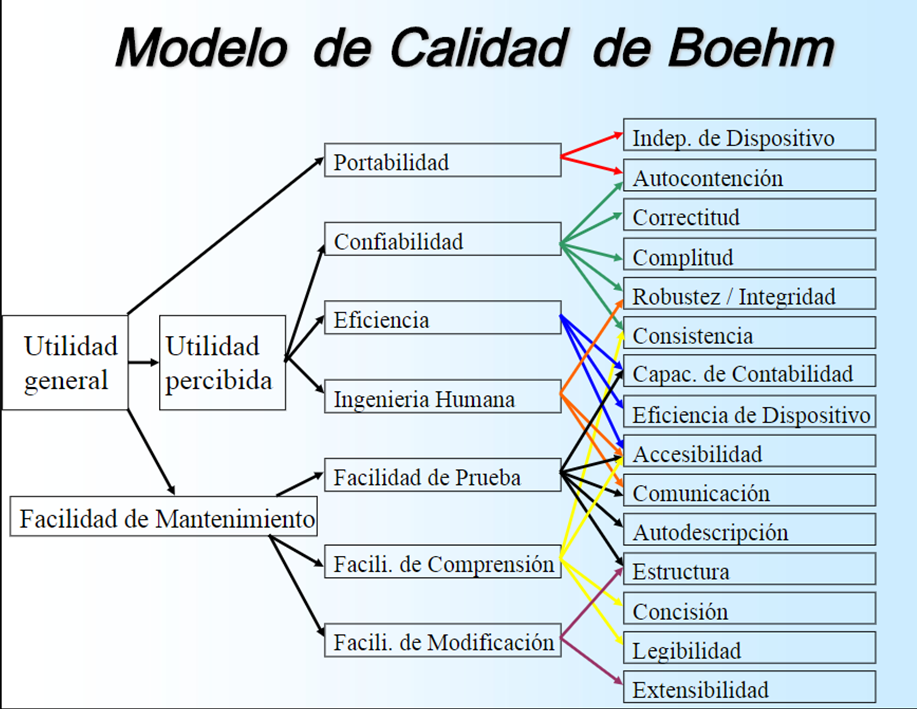
\includegraphics[width=0.6\textwidth]{Imagenes/boehmmmm.png}
    \caption{Relación entre componentes por capas}
    \label{fig:bohem1}
\end{figure}
\subsection{Ventajas del modelo}
El modelo de calidad propuesto por Barry Boehm presenta diversas ventajas que lo convierten en una herramienta sólida para la evaluación del software, ya que permite analizar de manera integral tanto las necesidades del usuario como los aspectos técnicos del sistema.
\begin{itemize}
    \item Permite una \textbf{evaluación estructurada}, ya que organiza la calidad del software en niveles (alto, intermedio y primitivo).
    \item Facilita la \textbf{comprensión del software}, al relacionar aspectos generales con detalles técnicos más específicos.
    \item Está \textbf{orientado al usuario}, considerando la utilidad, mantenibilidad y portabilidad como factores clave.
    \item Proporciona una \textbf{visión integral de la calidad}, incluyendo factores como eficiencia, usabilidad, fiabilidad y flexibilidad.
    \item Permite \textbf{medir la calidad}, gracias a sus características primitivas que se pueden asociar a métricas.
    \item Es flexible y adaptable a diferentes tipos de proyectos y etapas de desarrollo [11].
    \item Ayuda a \textbf{identificar fallos y debilidades} en el software de manera más precisa.
    \item Favorece la \textbf{mejora continua}, permitiendo realizar cambios, pruebas y mantenimiento con mayor facilidad.
    \item Es \textbf{flexible y adaptable}, ya que puede aplicarse a diferentes tipos de sistemas y proyectos.
    \item Apoya la \textbf{toma de decisiones}, al ofrecer criterios claros para evaluar y comparar productos de software.
    \item Puede utilizarse en \textbf{distintas etapas del desarrollo}, desde el diseño hasta la evaluación final.
\end{itemize}


\subsection{Desventajas del modelo}
El modelo de Boehm se limita bastante por la cantidad de características a tomar en cuenta, no define en cierta medida como debe cuantificarse ni tampoco expone en su totalidad como cada característica es utilizada
\begin{itemize}
    \item No se explica en muchos casos el cómo debe escogerse entre diferentes componentes o cómo priorizar una característica sobre otra.
    \item Con la gran cantidad de características a evaluar, se vuelve muy complejo probar cada una y es difícil definir la calidad en cada uno.
    \item No expone como realmente calcular la métrica medible o un valor para las características de eficiencia, exactitud, etc.
    \item Muchos de los modelos se centran en el lado del programador que del usuario, a pesar de tomar en cuenta accesibilidad y usabilidad, no detalla a la retroalimentación de los usuarios como una parte fundamental del modelo.
    \item Los niveles intermedios de Boehm no son los más detallados a comparación de los niveles altos y primitivos que al ser conceptos conocidos, el modelo jerárquico no ayuda a comprender tanto las relaciones como su utilidad en el modelo.
    \item En la actualidad, aunque los conceptos de calidad fueron muy bien diseñados, eran para sistemas de los años 70, no toma en cuenta factores como seguridad, interoperabilidad, microservicios, sincronía entre otras tecnologías modernas.
\end{itemize}

\subsection{Comparación con otros modelos de calidad}
El modelo de Boehm es muy cercano al modelo McCall ya que mantiene la jerarquía y el uso de características para evaluar la calidad de un producto. Sin embargo, considera en mayor medida al usuario y sus necesidades, ya que incluye el atributo de ingeniería humana que no estaba presente en el modelo de McCall, y coloca a las características que los usuarios perciben en el primer nivel. Esto permite establecer un mejor balance entre la calidad desde las perspectivas de clientes y desarrolladores.\\ \\
Por otra parte, si se compara con modelos más recientes, presenta algunas carencias. El modelo de Boehm es una de las principales influencias en la creación de los estándares ISO de calidad de software, incluido el 25010, ya que pasa las características del nivel medio a las características principales del ISO. Sin embargo, no toma en cuenta aspectos como la seguridad, que es crucial hoy en día, o la usabilidad, ya que si bien considera la perspectiva del usuario aún maneja atributos muy técnicos para medir su calidad en ese aspecto.

\subsection{Escenario Hipotético}
Una Fintech está migrando su sistema monolítico a una arquitectura de microservicios basada en la nube. El objetivo es asegurar que el nuevo sistema no solo funcione hoy (Utilidad Inicial), sino que sea fácil de mantener y migrar en el futuro (Utilidad a Largo Plazo), siguiendo la visión de Boehm.

\textbf{Aplicación de la Estructura Jerárquica:}
Para priorizar los atributos de calidad, aplicamos el modelo de arriba hacia abajo (enfoque descendente):
\subsubsection{Nivel 1 (Utilidad Global)}
El sistema debe procesar transacciones sin errores y permitir actualizaciones frecuentes sin interrumpir el servicio. Si el sistema no es "útil" bajo estas condiciones, el proyecto fracasa.
\subsubsection{Nivel 2 y 3 (Factores de Calidad)}
Seleccionamos tres de los siete factores de Boehm para este caso:
\begin{itemize}
    \item \textbf{Mantenibilidad (Modificabilidad)} \begin{itemize}
        \item \ul{Criterio:} Estructurabilidad;  Los microservicios deben estar desacoplados.
        \item \ul{Acción:} Evaluar si un cambio en el servicio de "Conversión de Moneda" afecta al servicio de "Auditoría".
    \end{itemize}
    \item \textbf{Mantenibilidad (Modificabilidad)} \begin{itemize}
        \item \ul{Criterio:} Independencia del Entorno.
        \item \ul{Acción:} El software debe poder moverse de un proveedor de nube (AWS) a otro (Azure) o a servidores locales si las regulaciones cambian.
    \end{itemize}
    \item \textbf{Mantenibilidad (Modificabilidad)} \begin{itemize}
        \item \ul{Criterio:} Precisión
        \item \ul{Acción:} Los cálculos de tasas e impuestos deben ser exactos según la normativa de cada país.
    \end{itemize}
\end{itemize}
\subsubsection{Nivel 4: Métricas Cuantitativas (Evaluación)}
Para que el modelo de Boehm sea efectivo, definimos métricas concretas:
\begin{table}[H]
    \centering
    \begin{tabular}{ |p{4cm}|p{6cm}|p{3cm}| }
        \hline
        \textbf{Factor} & \textbf{Métrica Sugerida} & \textbf{Meta} \\
        \hline
        \textbf{Mantenibilidad} & Tiempo medio de reparación (MTTR) & menor a 2 horas \\
        \hline
        \textbf{Portabilidad} & \% de código dependiente del sistema operativo   & 0\% (Uso de Docker)\\
        \hline
        \textbf{Fiabilidad} &Tasa de éxito de transacciones & 99.99\% \\
        \hline
        \textbf{Eficiencia}    &Tiempo de respuesta bajo carga máxima & Menor a 200ms \\
    \hline
    \end{tabular}
    \caption{Análiss de los atributos con métricas de calidad}
    \label{tab:aplicacion}
\end{table}
\subsubsection{Aplicación Práctica en el Ciclo de Vida}
Durante la fase de diseño, el equipo utiliza el modelo de Boehm para tomar una decisión crítica:
\begin{itemize}
    \item \textbf{Dilema: }¿Usar una base de datos propietaria muy rápida (Eficiencia) o una estándar compatible con múltiples sistemas (Portabilidad)?
    \item \textbf{Decisión bajo Boehm: }El modelo de Boehm otorga un peso significativo a la "Utilidad a largo plazo". El equipo decide sacrificar un 5\% de rendimiento por una mayor portabilidad, asegurando que el software pueda evolucionar y sobrevivir a cambios de infraestructura tecnológica, evitando el "vendor lock-in".
\end{itemize}
\subsubsection{Resultados del Análisis}
\begin{enumerate}
    \item \textbf{Priorización Clara: }Los desarrolladores saben que la legibilidad del código es más importante que la optimización extrema del CPU.
    \item \textbf{Trazabilidad: }Si una métrica falla (Nivel 4), se identifica inmediatamente qué factor de calidad (Nivel 2) está en riesgo y cómo afecta a la utilidad global (Nivel 1).
\end{enumerate}
\section{Conclusiones}
El modelo de Boehm es un modelo jerárquico con el fin de mejorar las falencias del modelo de McClall para la calidad de software,  clasifica los atributos de calidad por capas o niveles según su cercanía a una perspectiva de usuario o una perspectiva más técnica, no segmenta los principios, sino que define relaciones entre características y métricas de calidad que existen. Este enfoque permite realizar pruebas y correcciones especializadas en ciertos atributos para aumentar el nivel general de calidad, siendo tomado como referencia para otros estándares. Sin embargo, se debe aplicar de forma correcta ya que la estructura de atributos no es completamente sólida y al intentar cumplir objetivos de calidad muy específicos se pueden descuidar otros aspectos.
\section{Bibliografía}
{
    \sloppy
    \begin{enumerate}
    \item Boehm, B. W., Brown, J. R., \& Lipow, M. (1976). Quantitative evaluation of software quality. \textit{Software Engineering: Barry W. Boehm's Lifetime Contributions to Software Development, Management, and Research}, 25.
    \item Cano, M. A. (2025, octubre 7). Modelo de calidad del software de Boehm. \textit{Prezi}. https://prezi.com/p/hk5exv3xdy4s/modelo-de-calidad-del-software-de-boehm/
    \item Modelos Eredigitales. (2018, julio). El modelo de Boehm. \textit{Blogspot}. https://modeloseredigitales.blogspot.com/2018/07/el-modelo-de-boehm.html
    \item Professional QA. (s.f.). Boehm software quality model. https://www.professionalqa.com/boehm-software-quality-model
    \item Santhiya, S. (s.f.). \textit{SQM unit 1 and unit 2} [Presentación de diapositivas]. Scribd. https://www.scribd.com/presentation/64046141/SQM-Unit1-and-Unit-2
    \item Modelos de evaluación de recursos educativos digitales. (s.f.). \textit{Blogspot}. Recuperado el 29 de abril de 2026, de https://modeloseredigitales.blogspot.com/2018/07/el-modelo-de-boehm.html
    \item Modelos de Evaluación RED Grupo 9. (s.f.). Modelo de evaluación Boehm. \textit{Fandom Wiki}. https://modelos-de-evaluacion-red-grupo9.fandom.com/wiki/MODELO\_DE\_EVALUACION\_BOEHM
\end{enumerate}
}

%\newpage
%\input{Documento/2-Desarrollo}
%\newpage
%\input{Documento/3-Conclusiones}
%=================== Bibliografia ===================
\newpage
\addcontentsline{toc}{section}{Bibliografía}
\printbibliography[title={Bibliografía}] %Referencias
\end{document}